%%%%%%%%%%%%%%%%%%%%%%%%%%%%%%%%%%%%%%%%%
% 
% LaTeX Template
% Version 3.1 (25/3/14)
%
%%%%%%%%%%%%%%%%%%%%%%%%%%%%%%%%%%%%%%%%%

%----------------------------------------------------------------------------------------
%	PACKAGES AND DOCUMENT CONFIGURATIONS
%----------------------------------------------------------------------------------------

\documentclass[12pt, a4 paper]{article}

\usepackage{tikz}
%\usepackage[top=2cm, bottom=2cm, outer=0cm, inner=0cm]{geometry}
\usepackage{graphicx} % Required for the inclusion of images
\usepackage{multicol} % Required for multicolumns
\usepackage{setspace} % Required for line spacing
\setlength\parindent{0pt} % Removes all indentation from paragraphs
\setlength{\columnseprule}{0.4pt} % Adds vertical line between multicolumns
\usepackage{multirow} % Required for multirows
\usepackage{booktabs} % For prettier tables
\usepackage{ragged2e}
\usepackage{xcolor}
%\usepackage{tabularx}
%\renewcommand{\rmdefault}{ptm}

%\usepackage{helvet}

\usepackage{times} % Uncomment to use the Times New Roman font

%----------------------------------------------------------------------------------------
%	DOCUMENT INFORMATION
%----------------------------------------------------------------------------------------

\begin{document}

\tikz[remember picture,overlay] \node[inner sep=0pt] at (current page.center){
\includegraphics[width=\paperwidth,height=\paperheight]{image1.png}};

\clearpage

%\font\myfont=cmr12 at 35pt
%\title{\myfont  Event Name} % Write Event name here
%\author{}
%\date{\vspace{-10ex}}

%\maketitle % Insert the title, author and date
\setstretch{1}

\tikz[remember picture,overlay] \node[opacity=0.8,inner sep=0pt] at (current page.center){
\includegraphics[width=\paperwidth,height=\paperheight]{Border48-A4--Arvin61r58.png}};
%\tikz[remember picture,overlay] \node[opacity=0.5,inner sep=0pt] at (current page.center){\includegraphics[width=\paperwidth,height=\paperheight]{color-2174049__340.png}};

\begin{center}
\Huge \bfseries \ttfamily APTITUDE QUIZ
\end{center}

\begin{center}
\large A test based on technical questions
\end{center}

\begin{center}
\begin{multicols}{2}
\begin{tabular}{l r}
Date: & 05/04/2019\\ % Date the event was held
Time: & 3 P.M onwards \\ % Time of event 
\end{tabular}
\columnbreak
\begin{tabular}{l r}
Venue: & Mechanical Seminar Hall \\ % Venue of event
%Total Attendance: & Number \\ % Number of participants
\end{tabular}
\end{multicols}

\begin{Large}
%\begin{multicols}{2}
\justify
A Quiz based event ‘TECHNICAL APTITUDE QUIZ’ was organized by ISTE(INDIAN SOCIETY FOR TECHNICAL EDUCATION) in collaboration with SCIE and E2S2 on April 5,2019 in Mechanical Seminar Hall. 
%\columnbreak
%\includegraphics[width=\linewidth]{placeholder.jpg}
  %\caption{A boat.}
  %\label{fig:boat1}
%\end{multicols}

%\begin{multicols}{2}

%\includegraphics[width=\linewidth]{placeholder.jpg}

%\columnbreak
\justify
It was the first round –Selection Round for the Technical Aptitude Quiz.
%\end{multicols}


%\tikz[remember picture,overlay] \node[opacity=0.8,inner sep=0pt] at (current page.center){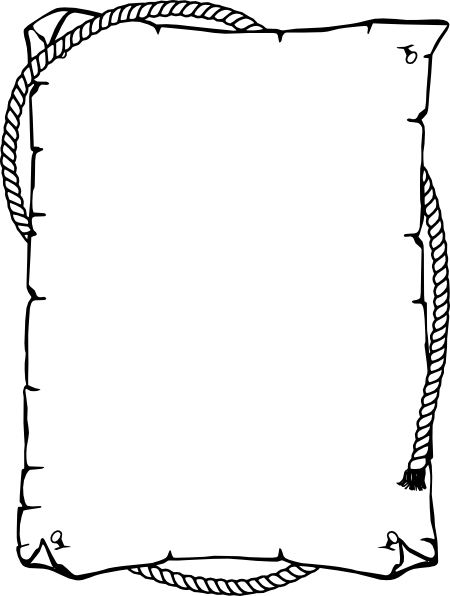
\includegraphics[width=\paperwidth,height=\paperheight]{5TRrp44jc.png}};
%\tikz[remember picture,overlay] \node[opacity=0.8,inner sep=0pt] at (current page.center){\includegraphics[width=\paperwidth,height=\paperheight]{md_5b0912b7c0870.png}};

%\begin{multicols}{2}
\justify
The event was mainly organized to test and improve the Aptitude of the students. The top 10participants were selected for the ‘Second Round of TECHNICAL APTITUDE QUIZ’. 
%\columnbreak
%\includegraphics[width=\linewidth]{placeholder.jpg}
  
%\end{multicols}

%\begin{multicols}{2}
%\includegraphics[width=\linewidth]{placeholder.jpg}

%\columnbreak

\justify
In the Selection Round the participants were provided with a set of 25 questions, which they were required to wind up in exact 25 minutes. Giving them one minute per question.
  
%\end{multicols} 

%\begin{multicols}{2}
\newpage
\justify
The cut o ff for the next round of ‘Technical Aptitude Quiz’ was set to be above score 15/25. Those 9 students whose score fit the criteria were promoted to the Round 2.

%\columnbreak
%\includegraphics[width=\linewidth]{placeholder.jpg}
  
%\end{multicols} 

%\begin{multicols}{2}
%\includegraphics[width=\linewidth]{placeholder.jpg}

%\columnbreak
\justify
The second round of ‘Technical Aptitude Quiz’ was the Qualifying Round, the selected students were provided with a set of 15 questions and were allotted a time of 10 minutes. The usage of cell phones was prohibited, neither the participants were allowed to discuss while the quiz was going on.
  
%\end{multicols} 

\end{Large} 
\end{center}

\tikz[remember picture,overlay] \node[opacity=0.8, inner sep=0pt] at (current page.center){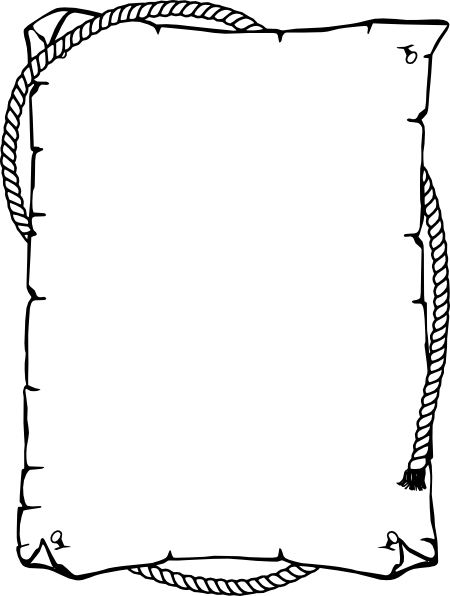
\includegraphics[width=\paperwidth,height=\paperheight]{5TRrp44jc.png}};
%\tikz[remember picture,overlay] \node[opacity=0.8,inner sep=0pt] at (current page.center){\includegraphics[width=\paperwidth,height=\paperheight]{md_5b0912b7c0870.png}};

\newpage

\tikz[remember picture,overlay] \node[opacity=0.8, inner sep=0pt] at (current page.center){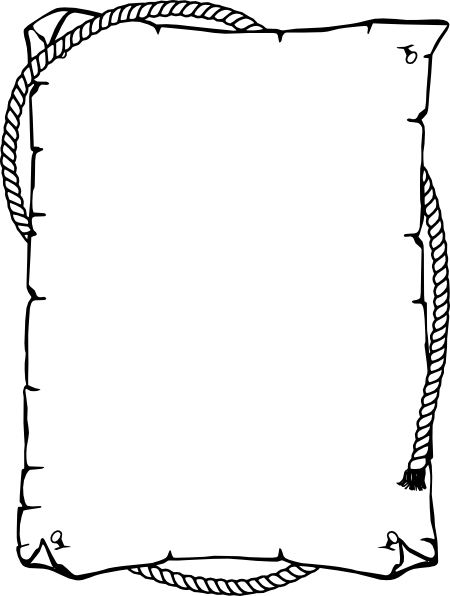
\includegraphics[width=\paperwidth,height=\paperheight]{5TRrp44jc.png}};

\begin{center}
\Huge Pictures Section

\medskip

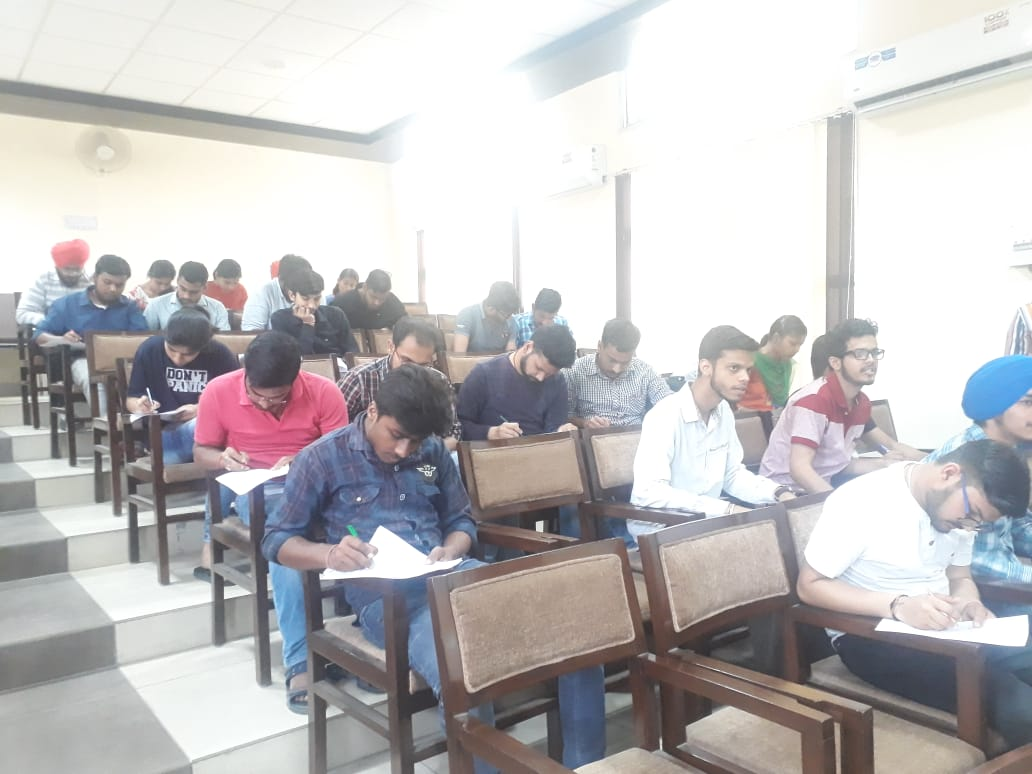
\includegraphics[height=6cm]{image2.jpg}
\medskip

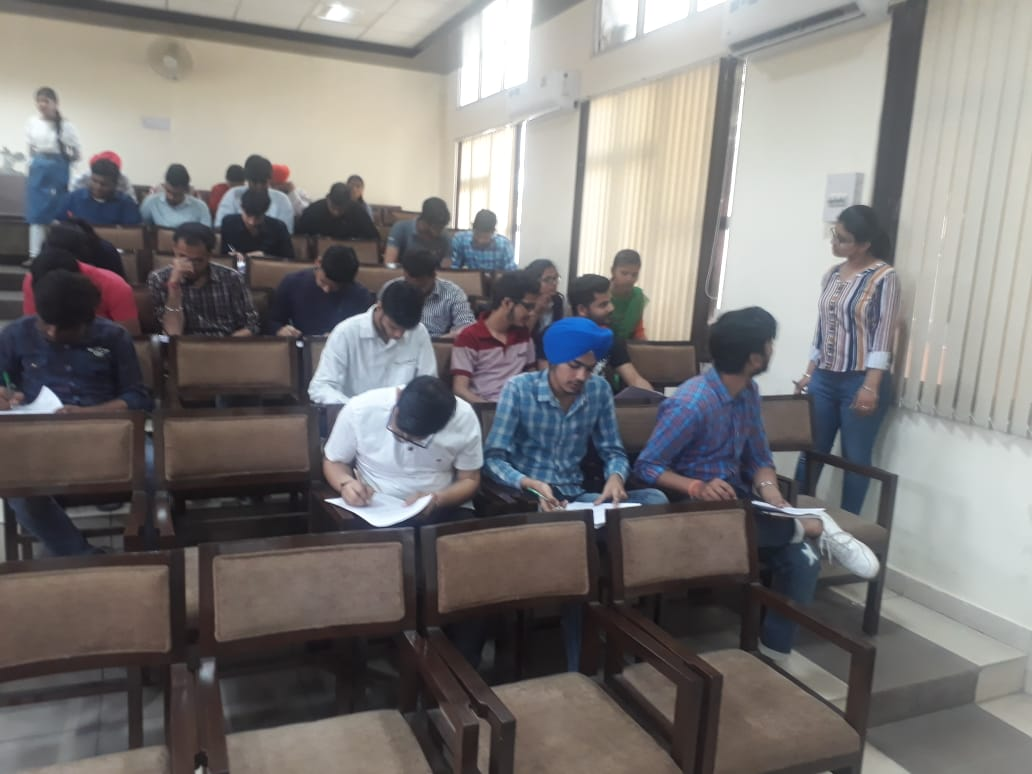
\includegraphics[height=6cm]{image3.jpg}
\medskip

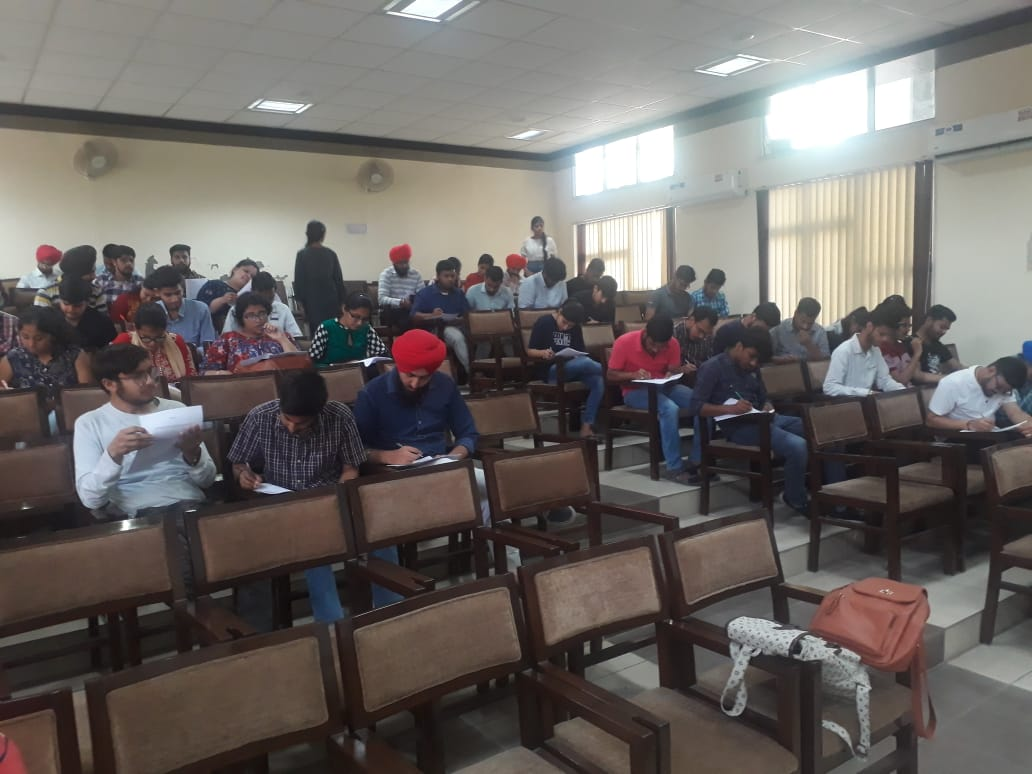
\includegraphics[height=6cm]{image4.jpg}
\begin{center}

\end{center}


\huge Organisers list
\end{center}

\begin{table}[h!]
  \begin{center}
    \begin{tabular}{|c|c|c|c|c|c|} 
    \toprule % <-- Toprule here
      \textbf{S.No.} & \textbf{Name} & \textbf{Branch/Year} & \textbf{Roll No.} \\
      \midrule % <-- Midrule here
      1 & KIRT PREET SINGH & D2 ECE	& 1706741 \\
      2	& TUSHAR CHAUHAN   & D2 ME	& 1706533 \\
      3	& MANPREET	       & D2 CSE	& 1706471 \\
      4	& ALOK	           & D2 ME	& 1706945 \\
      5	& PAWANDEEP SINGH  & D4 CSE	& 1507637 \\
      6	& JATIN TYAGI	   & D4 ECE	& 1507883 \\
      7	& BINAY RANJAN	   & D4 ME	& 1508229 \\
      8	& VISHAL RAJ	   & D3 PE	& 1607467 \\

      \bottomrule % <-- Bottomrule here
    \end{tabular}
  \end{center}
\end{table}


\tikz[remember picture,overlay] \node[opacity=0.8,inner sep=0pt] at (current page.center){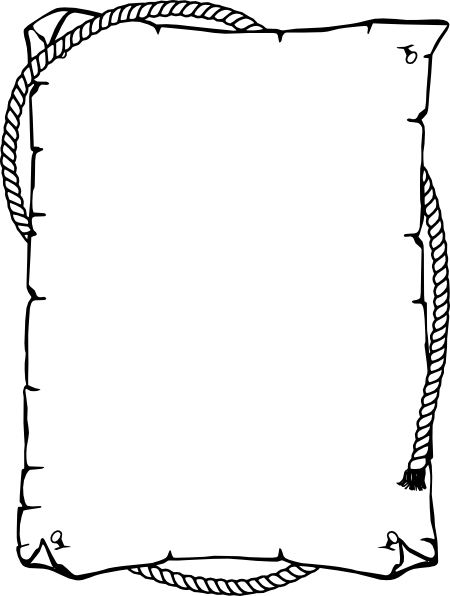
\includegraphics[width=\paperwidth,height=\paperheight]{5TRrp44jc.png}};
%\tikz[remember picture,overlay] \node[opacity=0.8,inner sep=0pt] at (current page.center){\includegraphics[width=\paperwidth,height=\paperheight]{md_5b0912b7c0870.png}};

\begin{center}
\huge Winners List
\end{center}

\begin{table}[h!]
  \begin{center}
    \begin{tabular}{|c|c|c|c|c|c|} 
    \toprule % <-- Toprule here
      \textbf{S.No.} & \textbf{Name} & \textbf{Branch/Year} & \textbf{Roll No.} &\textbf{Position} \\
      \midrule % <-- Midrule here
      1 & HARSHIT	    & D3 EE	 & 1606823 & 1st \\
      2	& HARDEEP SAINI	& D3 EE	 & 1606852 & 2nd \\
      3	& ACHINTYA	    & D2 CSE & 1706390 & 3rd \\

      \bottomrule % <-- Bottomrule here
    \end{tabular}
  \end{center}
\end{table}


\end{document}